%%%%%%%%%%%%%%%%%%%%%%%%%%%%%%%%%%%%%%%%%%%%%%%%%%%%%%%%%%%%%%%%%%%%%%
%%                     Logic arc
%%%%%%%%%%%%%%%%%%%%%%%%%%%%%%%%%%%%%%%%%%%%%%%%%%%%%%%%%%%%%%%%%%%%%%

\subsection{Glyph: \glyph{Logic arc} }\label{sec:logicArc}

\glyph{Logic arc} is used to represent the fact that an activity influences the outcome of a logic operator.

\begin{glyphDescription}
 \glyphSboTerm SBO:0000398 ! logical relationship.
 \glyphOrigin Any \glyph{Activity node} (\sect{af:ANs}) or any \glyph{logical operator} (\sect{af:logic}).
 \glyphTarget Any \glyph{logical operator} (\sect{af:logic}).
 \glyphEndPoint No particular symbol is used to represent a logic arc.
 \end{glyphDescription}

\begin{figure}[H]
  \centering
  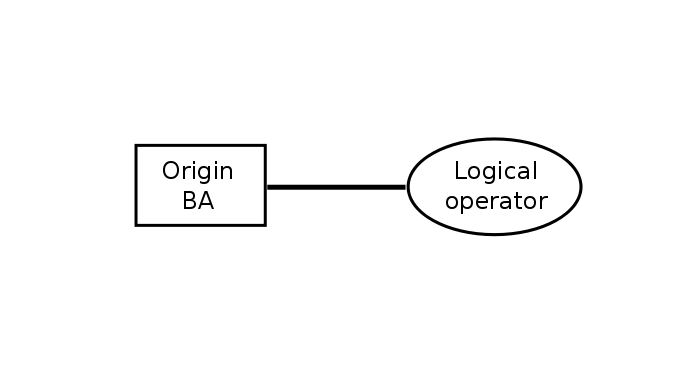
\includegraphics[scale = 0.4]{images/logicArc}
  \caption{The \AF glyph for \glyph{logic arc}.}
  \label{fig:logicArc}
\end{figure}
